\documentclass[border=5pt]{standalone}
\usepackage{tikz}
\usepackage{amsmath}
\usetikzlibrary{patterns, positioning}

\begin{document}

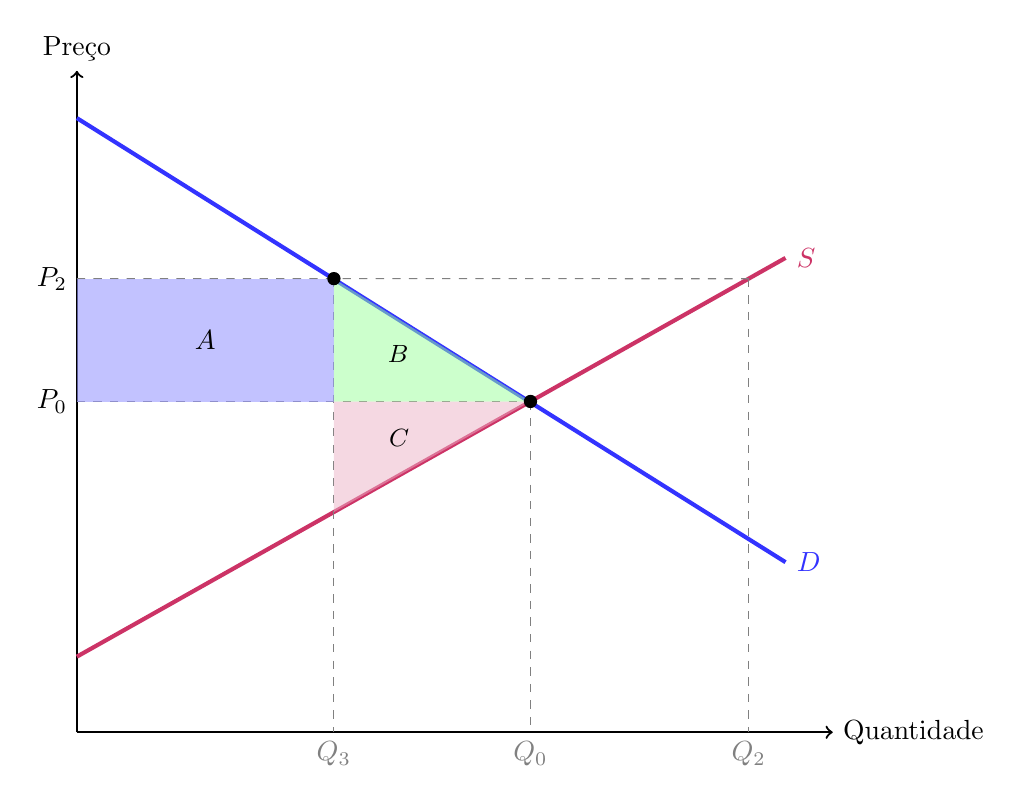
\begin{tikzpicture}[scale=1.2]
    % Eixos
    \draw[thick, ->] (0,0) -- (8,0) node[right] {Quantidade};
    \draw[thick, ->] (0,0) -- (0,7) node[above] {Preço};
    
    % Curva de Demanda (D) - ajustada para novo equilíbrio em (4.8, 3.5)
    % y = 6.5 - 0.625*x
    \draw[thick, blue!80, line width=1.5pt] (0,6.5) -- (7.5,1.8) node[right] {$D$};
    
    % Curva de Oferta (S) - inicia no eixo vertical (0, 0.8) e passa por (4.8, 3.5)
    % y = 0.8 + 0.5625*x
    \draw[thick, purple!80, line width=1.5pt] (0,0.8) -- (7.5,5.02) node[right] {$S$};
    
    % Interseção (equilíbrio de mercado) - movido para a direita
    \coordinate (E) at (4.8,3.5);
    
    % Preço de equilíbrio
    \coordinate (P0) at (0,3.5);
    \draw[dashed, gray] (P0) -- (E);
    \draw (0,3.5) node[left] {$P_0$};
    
    % Preço mínimo (acima do equilíbrio) - mantém proporção
    \coordinate (P2) at (0,4.8);
    
    % Calcular Q3 e Q2 corretamente
    % Q3: interseção de P2=4.8 com demanda D: 4.8 = 6.5 - 0.625*x => x = 2.72
    % Q2: interseção de P2=4.8 com oferta S: 4.8 = 0.8 + 0.5625*x => x = 7.11
    \coordinate (D2) at (2.72,4.8);
    \coordinate (S2) at (7.11,4.8);
    
    \draw[dashed, gray] (P2) -- (7.11,4.8);
    \draw (0,4.8) node[left] {$P_2$};
    
    % Quantidades - Q3 e Q2 corrigidos
    \draw[dashed, gray] (2.72,4.8) -- (2.72,0) node[below] {$Q_3$};
    \draw[dashed, gray] (4.8,3.5) -- (4.8,0) node[below] {$Q_0$};
    \draw[dashed, gray] (7.11,4.8) -- (7.11,0) node[below] {$Q_2$};
    
    % Área A (retângulo - transferência de excedente do consumidor) - mais comprido
    \fill[blue!40, opacity=0.6] (0,3.5) rectangle (2.72,4.8);
    \node at (1.36,4.15) {$A$};
    
    % Triângulo B (acima do preço P0 e abaixo da curva de demanda)
    % Pontos: (2.72, P2=4.8), (4.8, P0=3.5), (2.72, P0=3.5)
    % Forma um triângulo entre Q3, Q0 e a curva de demanda
    \fill[green!40, opacity=0.5] (2.72,4.8) -- (4.8,3.5) -- (2.72,3.5) -- cycle;
    \node at (3.4,4.0) {\small $B$};
    
    % Triângulo C (acima da curva de oferta e abaixo do preço P0)
    % Pontos: (2.72, na oferta), (2.72, P0=3.5), (4.8, P0=3.5)
    % Oferta em x=2.72: y = 0.8 + 0.5625*2.72 = 2.33
    % Centro do triângulo: ((2.72+2.72+4.8)/3, (2.33+3.5+3.5)/3) = (3.41, 3.11)
    \fill[purple!30, opacity=0.5] (2.72,2.33) -- (2.72,3.5) -- (4.8,3.5) -- cycle;
    \node at (3.41,3.11) {\small $C$};
    
    % Pontos principais
    \fill (E) circle (2pt);
    \fill (D2) circle (2pt);

\end{tikzpicture}

\end{document}
